\section{Motivation and Significance}\label{motivation-and-significance}

In previous work, Billings et. al., discovered through requirements
gathering interviews that many of the difficulties using
high-performance modeling and simulation software fall broadly into five
distinct categories, \cite{billings_designing_2009}. These activities,
detailed in section \ref{workflow-model}, include (1) creating input,
(2) executing jobs, (3) analyzing results, (4) managing data, and (5)
modifying code. There are many tools that address these problems
individually, but the same research found that the excess number and
specialization of these tools also contribute to the learning curve.

Efforts to address these five issues have previously resulted in general
purpose scientific workflow tools like Kepler, 
\cite{ludascher_scientific_2006}, or myopic tools that only satisfy a single
set of requirements for a single piece of software or platform. These
are opposing extremes, but a middle-of-the-road solution is also
possible. A workflow engine could be developed that limits its scope to
high-performance computing (HPC) and to the set of possible workflows
associated with the five previously mentioned activities. With only
minor additional development, a rich application programming interface
(API) could be exposed so that highly-customized solutions could still
be made based on this limited workflow engine.

It is not clear which, if any, of these solutions is better than the
others, and practical requirements will ultimately dictate the path of a
project's progress. This work considers a middle ground solution and
presents the Eclipse Integrated Computational Environment (ICE) as proof
that it is possible to create such a system. Specifically, the work
described here shows that:

\begin{itemize}
\item
  Modeling and simulation activities can be described in a succinct
  workflow model, (see ``Workflow Model'').
\item
  An architecture for such a workflow system can satisfy the model of
  workflows in an extensible way, (see ``Software Architecture'').
\item
  Such a system is applicable to a suite of problems in energy science,
  including virtual battery simulations, additive manufacturing and
  other areas, (see ``Illlustrative Examples'').
\end{itemize}

This section concludes with an introduction of the workflow model addressed by
ICE. Section \ref{software-description} presents the details of the software
from an architecture perspective while section \ref{illustrative-examples}
provides a set of comprehensive examples. Finally, this paper concludes with a
presentation of the impact, (section \ref{impact}), and sample code,
(section \ref{sample-code-tutorials-and-other-resources}).

\subsubsection{Workflow Model}\label{workflow-model}

Computational scientists perform a variety of tasks in modeling and
simulation that can be abstracted into a lightweight theoretical
framework based broadly on five high-level \emph{activities}: (1)
creating input, (2) executing jobs, (3) analyzing results, (4) managing
data, and (5) modifying code. Those same computational scientists would
most likely find these activities difficult for all codes with which
they lack experience, whereas with their own codes---or those with which
they are most familiar---these tasks may be so simple that they are
taken for granted. Any particular combination of these activities across
one or more scientific software package or code results in a unique
\emph{workflow}. Such a workflow is normally, but not always, requested
by a human user and orchestrated by a \emph{Workflow Management System
(WMS)}.

The most obvious workflow for any individual simulation code or
collection of codes is to string the activities together: the user's
workflow is to create the input, launch the job, perform some analysis,
and manage the data---possibly modifying the code in the process. There
are many other combinations however, including re-running jobs with
conditions or modifications or analyzing someone else's data (See
footnote 1).\footnote{The
authors have identified many different combinations of these activities that
define workflow ``classes.'' When possible, every effort is made to give the
classes funny names such as ``The Re-Run'' or ``The Graduate Student.''}

\textbf{Creating input} is the process of describing the physical model
or state of a system that will be simulated. This could include creating
an input file(s) or making calls to an external process to configure a
running program. In most situations, a computational scientist will
modify existing input or create new input from a template. ``Input''
generally includes runtime parameters for the simulation framework
(e.g., tolerances); configuration options (e.g., data locations, output
locations, module configurations); properties of the materials to be
simulated; and a discretization of the simulation space (e.g., mesh,
grid, particle distribution). The collection of all required input can
be quite large and may go by many names, including ``input set,''
``input package,'' ``problem,'' or, simply, ``input.'' Often, the set of
input files will be described in a ``main'' input file that acts as a
kind of manifest, describing and providing links to all necessary
information for a given problem.

In this work, it should be assumed---unless otherwise noted---that
``input'' refers to the entire set of input, not to a single file.

\textbf{Executing jobs}, or ``running the workflow'' in this context, is
the process of performing calculations using a simulation code or
framework based on known variables---the input. Models and simulation
codes are typically run locally for small jobs or for development. Large
simulations, on the other hand, typically require a large amount of
hardware resources; these resources are usually off site (i.e.,
physically unavailable to the user) and are accessed remotely
through Secure Shell (SSH) connections or similar protocols. Remote
execution requires moving the input in advance of the execution and
copying or moving the output to the user's machine. In many cases,
though, the output is too large to move to the user's local machine.

Local and remote jobs are often monitored to ascertain a job's status.
This monitoring may be a simple check as to whether or not the execution
has completed, or it may involve monitoring the output of individual
quantities to examine the calculation state. The latter is often used to
detect calculation errors that will result in incorrect results. If such
problems are found, the job is typically cancelled (``killed'') to save
compute resources and is then re-run later.

In this work, it should be assumed---unless otherwise noted---that
``executing a job'' includes monitoring that job in one or more ways,
possibly including real-time updates to visualizations.

\textbf{Analyzing results} includes executing special jobs to transform
data in one or more prescribed ways and producing artifacts with
scientific significance from the transformed data. This may include, for
example, post-processing results and visualizing the new data with
dedicated visualization tools. For many types of scientific computing,
this includes viewing the results of a simulation on a mesh or grid and
extracting publication quality images or movies from that data. Other
cases may include analyzing results in preparation for follow on
simulations or performing feature extraction, classification, or
activities for machine learning and data mining.

While this has many similarities to executing a job, it is distinctly
different because the activity changes focus to satisfy the needs of a
human operator. Simple data reduction, where the exact reduction is
known, certainly qualifies as executing a job; however, analysis of
model and simulation results is far from simple data reduction, and is
generally far more interactive for computational scientists.

\textbf{Managing data} includes moving, copying, storing, sharing, or
otherwise interacting with data for or from simulations. This activity
is the most pervasive because each of the other activities requires
interacting with data in some way. In many cases, though, data is still
managed for its own purposes, without performing a simulation,
generating new input, or analyzing results. Examples include archiving
data, packaging data for publications, and updating values manually
(often in light of new information from publications).

\textbf{Modifying code} is not typically considered a part of a
scientific computing workflow. However, modeling and simulation use
cases often require users to explicitly modify code before execution,
such as with the computational fluid dynamics code Nek5000,
\cite{the_nek5000_team_nek5000_2014}, or to issue special re-build instructions.
Many computational scientists consider ``their workflow'' to be re-running
software after modifications for purely exploratory purposes. This may
be required if the model that the author is manipulating cannot be
configured directly as part of the input but can be easily manipulated
by hand.

\subsubsection{Comparison to Other
Models}\label{comparison-to-other-models}

This model of workflows differs significantly from those of similar
efforts in workflow science because it defines workflows in terms of
activities. Other workflow models in the literature define a workflow as
a collection of computing processes. For example, Yu and Buyya define
grid workflows as ``a collection of tasks that are processed on
distributed resources in a well-defined order to accomplish a specific
goal,'' \cite{yu_taxonomy_2005}. Others, such as Pizzi et al., subscribe to
similar definitions, \cite{pizzi_aiida:_2016}. This ``process'' view is
acceptable where the workflow is static and does not require additional
human input or ``human in the loop'' behavior after the all the initial
human input is provided. That is, a ``process-oriented'' definition is
acceptable where all human input is provided in advance. However,
workflows within ICE are fully interactive with regular call-backs to
humans. It is simpler to discuss ``activities'' than it is to create a
distinction between ``human processes'' and ``computer processes.''
Focusing on ``activities'' over processes (human or computer) also has
the benefit of removing concrete elements such as hardware properties or
software details that distract from details of workflows and WMSes. That
is, considerations such as memory usage and raw performance are
important, but questions about the abstract workflow or what the WMS
should do are far more important.

\section{Software Description}\label{software-description}

ICE was specifically created to address the workflow model described
above, which is to say that it was created specifically to address
hands-on workflows for computational scientists. Users download and
execute ICE locally and it orchestrates workflows locally or remotely as
required. It provides a comprehensive workbench for modeling and
simulation that includes tools for workflows, visualization, data
management, and software development.

\subsection{Software Architecture}\label{software-architecture}

Workflows and tasks in ICE are not explicitly treated as trees -
Directed Acyclic Graphs, (DAGS) - as is common with grid workflow tools,
\cite{yu_taxonomy_2005}. Instead, ICE's design is inspired by Representational
State Transfer (REST), \cite{fielding_architectural_2000}.

Users initiate requests to create, edit, update or delete workflows from
the \emph{ICE Client} (the workbench). The list of available workflows
that can be created is provided dynamically to the \emph{ICE Client} by
the \emph{ICE Core}, which acts as a server. This information is
provided dynamically since it often changes at run time based on the
configuration of available workflow components in the registry and on
persisted workflows that users have saved in their workspace.
Information about workflows are provided from the Core to the Client
through \emph{stateless Forms} that describe the workflow and provide
all the necessary information to understand \emph{what} should process
the workflow, (but not \emph{how} it should be processed). Once users
modify the description of the workflow in the Form to provide their
specific details, the Client dispatches a request to the Core to modify
or process the workflow. The Core then uses the information in the Form
to perform a service lookup for \emph{what} should process the workflow.

Workflows in ICE are encoded in and processed by \emph{Items} and each
workflow type is a subclass of Item. Items are registered dynamically
through a service registry in ICE, (see section \ref{framework}), and
provide the Forms for the ICE Core and Client. Since ICE's design is
highly object oriented, it is easiest to think of the Item class as a
description of an abstract workflow and an Item object (an instance of
the class) as a concrete workflow with all required execution details
provided by its Form.

Individual components of workflows, i.e. - workflow ``tasks'' or
``nodes'' - are either encoded directly in the workflow's subclass of
Item or provided as \emph{Actions} that are dynamically registered with
an \emph{Action Factory} and obtained at runtime. Table 1. describes the
differences between Items, Actions, and Forms.\footnote{An upcoming update to the API will see the formal introduction of
IWorkflow, IWorkflowTask, and IWorkflowEngine interfaces to bring ICE's
API language closer to other systems. This must be done with care to
satisfy backwards compatibility requirements on the present API.}

\begin{table*}[t]
\begin{tabularx}{\textwidth}{|l|X|l|}
\hline
Class & Class Description & Object Description\tabularnewline\hline
Item & Java class with code to execute an abstract workflow. Provides a
Form. & Concrete workflow executor.\tabularnewline\hline
Form & Description and template of the data needed for the Item to
process the workflow. & User-modified workflow data.\tabularnewline\hline
Action & Java class for executing a specific task in the workflow. Used
by Items. & Concrete workflow task executor.\tabularnewline\hline
\end{tabularx}
\caption{Class Descriptions for Items, Forms and Actions}
\end{table*}

In addition to running as a desktop workbench, ICE can be run as a
headless web server with a remote service interface and a web
Application Programming Interface (API). The web API is also used as the
primary means of providing real-time feedback and monitoring support in
ICE.

\subsubsection{Item States}\label{item-states}

All Items in ICE are finite state machines where the states represent
the abstract state of the workflow. For example, when an Item is first
created, it enters the ``Form Ready'' state to indicate that it could,
in theory, be processed after a user reviews it. After that review it
enters the ``Ready to Process'' state before and the ``Processed'' state
after it is processed. There are several additional states for errors.

This design is very important. First, it means that all workflows in
ICE, regardless of their actual details and function, can only behave in
a specific set of known, predictable ways. This greatly simplifies the
way that the Core manages and interacts with Items. Second, it
explicitly delineates which workflows can be executed from those that
must still receive some configuration because it formalizes state and
error checks. Finally, it allows developers implementing Items and
Actions to specify by contract what is required before proceeding to the
next task, processing the workflow, or declaring a successful execution.

\subsubsection{Persistence and
Workspaces}\label{persistence-and-workspaces}

ICE persists permanent copies of Forms to disk when workflows are
created and modified in a special directory called a \emph{workspace}.
Workspaces can contain projects, folders and files, including data,
code, input and output. ICE automatically manages local and remote (or
even local \emph{to} remote) transfers of data files when executing
workflows if the files are detected in the same directory of the
workspace as the workflow itself. For example, when executing a remote
job, ICE will automatically move the input file if it is specified in
the workflow and available in the project directory of the workspace.
Likewise, if output is small enough, ICE will automatically move it back
to local directory. By convention, all paths in ICE's Forms are
relative to the workspace root path. Workspace directories are specified
by the user.

ICE handles persistence using a \emph{persistence provider}. The only
default persistence provider uses JAX-RS, \cite{burke_restful_2010}, to write
Forms to XML. In principle other persistence providers could replace the
XML-based provider since it is registered as a dynamic service, and in
the past a JAX-P based provider has been used.

\subsubsection{Extending the Framework to Add Custom
Workflows}\label{framework}

ICE is an Eclipse Rich Client Platform (RCP) application,
\cite{mcaffer_eclipse_2010}. It has a plugin architecture based on Equinox, the
reference implementation of the Open Service Gateway Initiative (OSGi) framework specification, \cite{mcaffer_osgi_2010}. It uses over 1200 additional
packages from the Eclipse ecosystem to provide services such as language
support and visualization to users. Each unique element of ICE described
in this work, including the client, core, all Items, data structures and
many others are provided as plugins to Equinox. Most plugins are
dynamically managed and provided as services that can be obtained from a
service registry. All file I/O in ICE, with only a few exceptions,
interacts with the RCP's Resources plugin. This includes remote
resources that are managed with the Eclipse Parallel Tools Platform,
\cite{tibbitts_integrated_2009}.

It is not possible to graphically create new Items in ICE. Users can
only use the workflow Items provided with their version of ICE unless
they provide their own plugin to the framework. This can seem like an
onerous task to the novice user especially if they do not know Java, but
this design was chosen because it is, in the opinion of the authors, a
far more sophisticated and sustainable way to create workflows than
through wiring diagram.

ICE provides built-in development tools to auto-generate ``stubs'' of
plugins that can then be installed into the framework. This
``self-hosting'' makes it possible for new users to create complex,
sophisticated workflows very quickly because they are not required to
know how to interact with the framework. Furthermore, ICE provides a
rich API, documentation, tutorials, and tools to further simply the
process.

There are many situations where graphically configuring workflows is
unacceptable, such as when a very large number of workflows will be
executed or the type of information required is very fine-grained. In
these cases, it is often necessary to provide scripts to the workflow
management system. ICE includes the Eclipse Advanced Scripting
Environment, \cite{pontesegger_eclipse_2015}, (EASE), for scripting because it
provides a native way to script Eclipse RCP projects in Javascript,
Jython, and Python. This also makes it possible to extend the
environment by adding Items in these languages.

\subsection{Software Functionalities}\label{software-functionalities}

The most important function of ICE is to serve as an easily extended
workflow management system for computational scientists in support of
the activities described above. In practice, it is most often used as a
combination of workflow management system and development environment
since it contains a significant amount of Eclipse's software development
tooling in addition to the workflow tools. The project has many users,
but it is most heavily used by the development team to support workflow
science and software development for energy science projects. The
development team regularly uses the platform to quickly deploy new
domain-specific workbenches in a matter of hours for small collections
of workflows that are easy to encode.

Outside of the development team, ICE is commonly deployed as a
sophisticated user environment for computational science projects (see
``Impact'' below) and as a visualization tool. The ICE source code originally contained a
significant amount of visualization support, but at the request of users
in the community that support was ``spun off'' in early 2016 as a
separate visualization project, the Eclipse Advanced Visualization
Project, EAVP, \cite{billings_eclipse_2015}.

\section{Illustrative Examples}\label{illustrative-examples}

The role that ICE plays as a workflow tool is best illustrated by the
various ways that it has been deployed.

\subsection{Virtual Battery
Simulations}\label{virtual-battery-simulations}

Pannala et al. developed a Virtual Integrated Battery Environment (VIBE)
as part of their research into safety and performance characteristics of
lithium ion batteries, \cite{pannala_multiscale_2015}. VIBE provides ICE to
users as part of its distribution. New workflows were added to ICE to create
multiple types of input, configure the simulation software, and launch
simulations of virtual batteries. Interactive 3D visualizations of the
results were embedded in the launcher so that users would quickly find
their results. Figure 1 shows the results from a temperature
distribution of a prismatic cell battery simulated during discharge.

\begin{figure}[htbp]
\centering
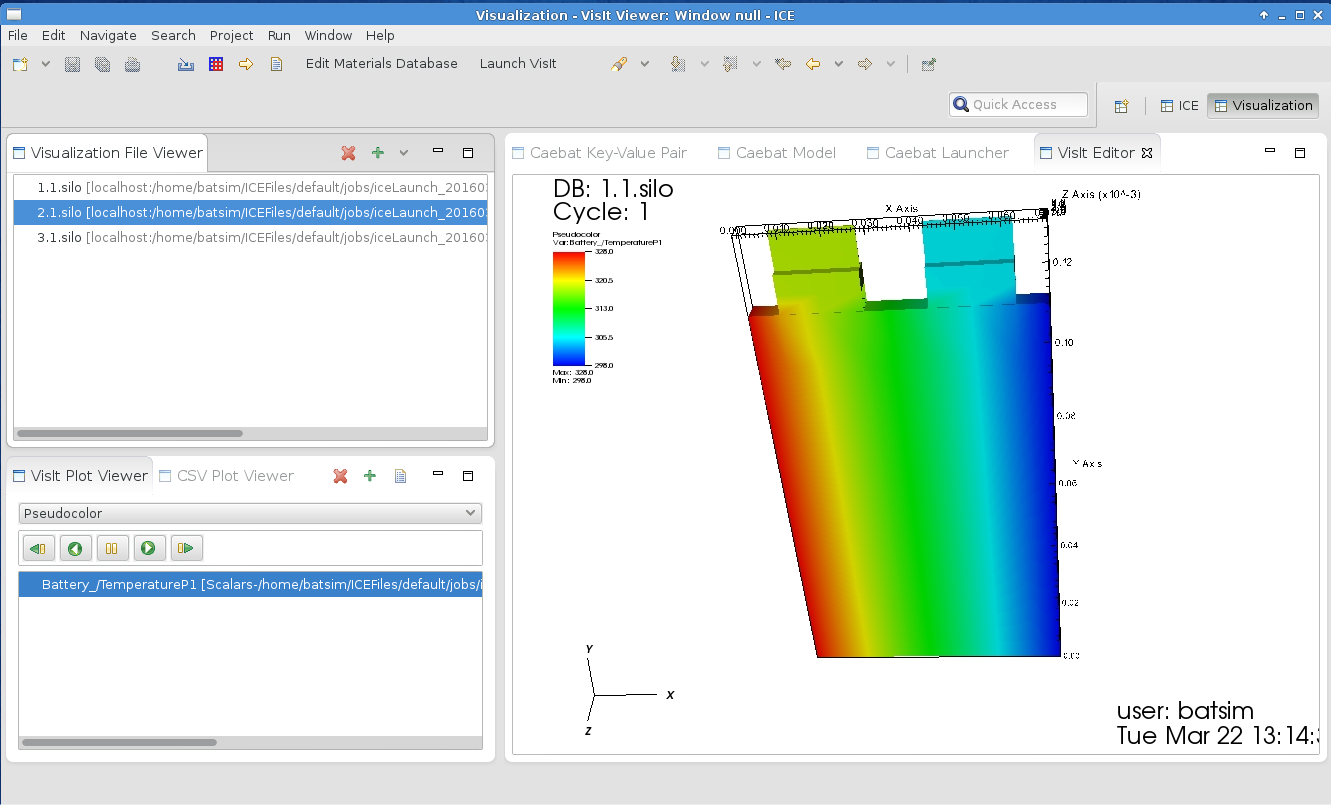
\includegraphics[width=\textwidth]{images/vibe_20151016.png}
\caption{ICE workbench for VIBE analysis.}
\end{figure}

VIBE 1.0 is available as a virtual machine in which the simulation
software and ICE are provided side by side. More recent efforts for VIBE
1.1 by the VIBE development team include providing the simulation
software in Docker containers so that users can download the latest,
native version of ICE for their machine while simultaneously benefiting
from a smaller virtual machine for the simulator.

\subsection{Multiphysics Simulations with
MOOSE}\label{multiphysics-simulations-with-moose}

The MOOSE Framework is a powerful, easy to use multiphysics framework
developed at the Idaho National Laboratory, \cite{gaston_moose:_2009}. ICE
provides workflow tools for MOOSE as well as specialized class
generation utilities for developing custom MOOSE kernels. Many of the
MOOSE tools in ICE were developed closely with the MOOSE team to closely
reproduce various aspects of MOOSE's user interface, Peacock. Figure 2
shows an example of the ICE workbench for a simple structural mechanics
problem solved with the MOOSE framework, \cite{mccaskey_scientific_2015}.

\begin{figure}[htbp]
\centering
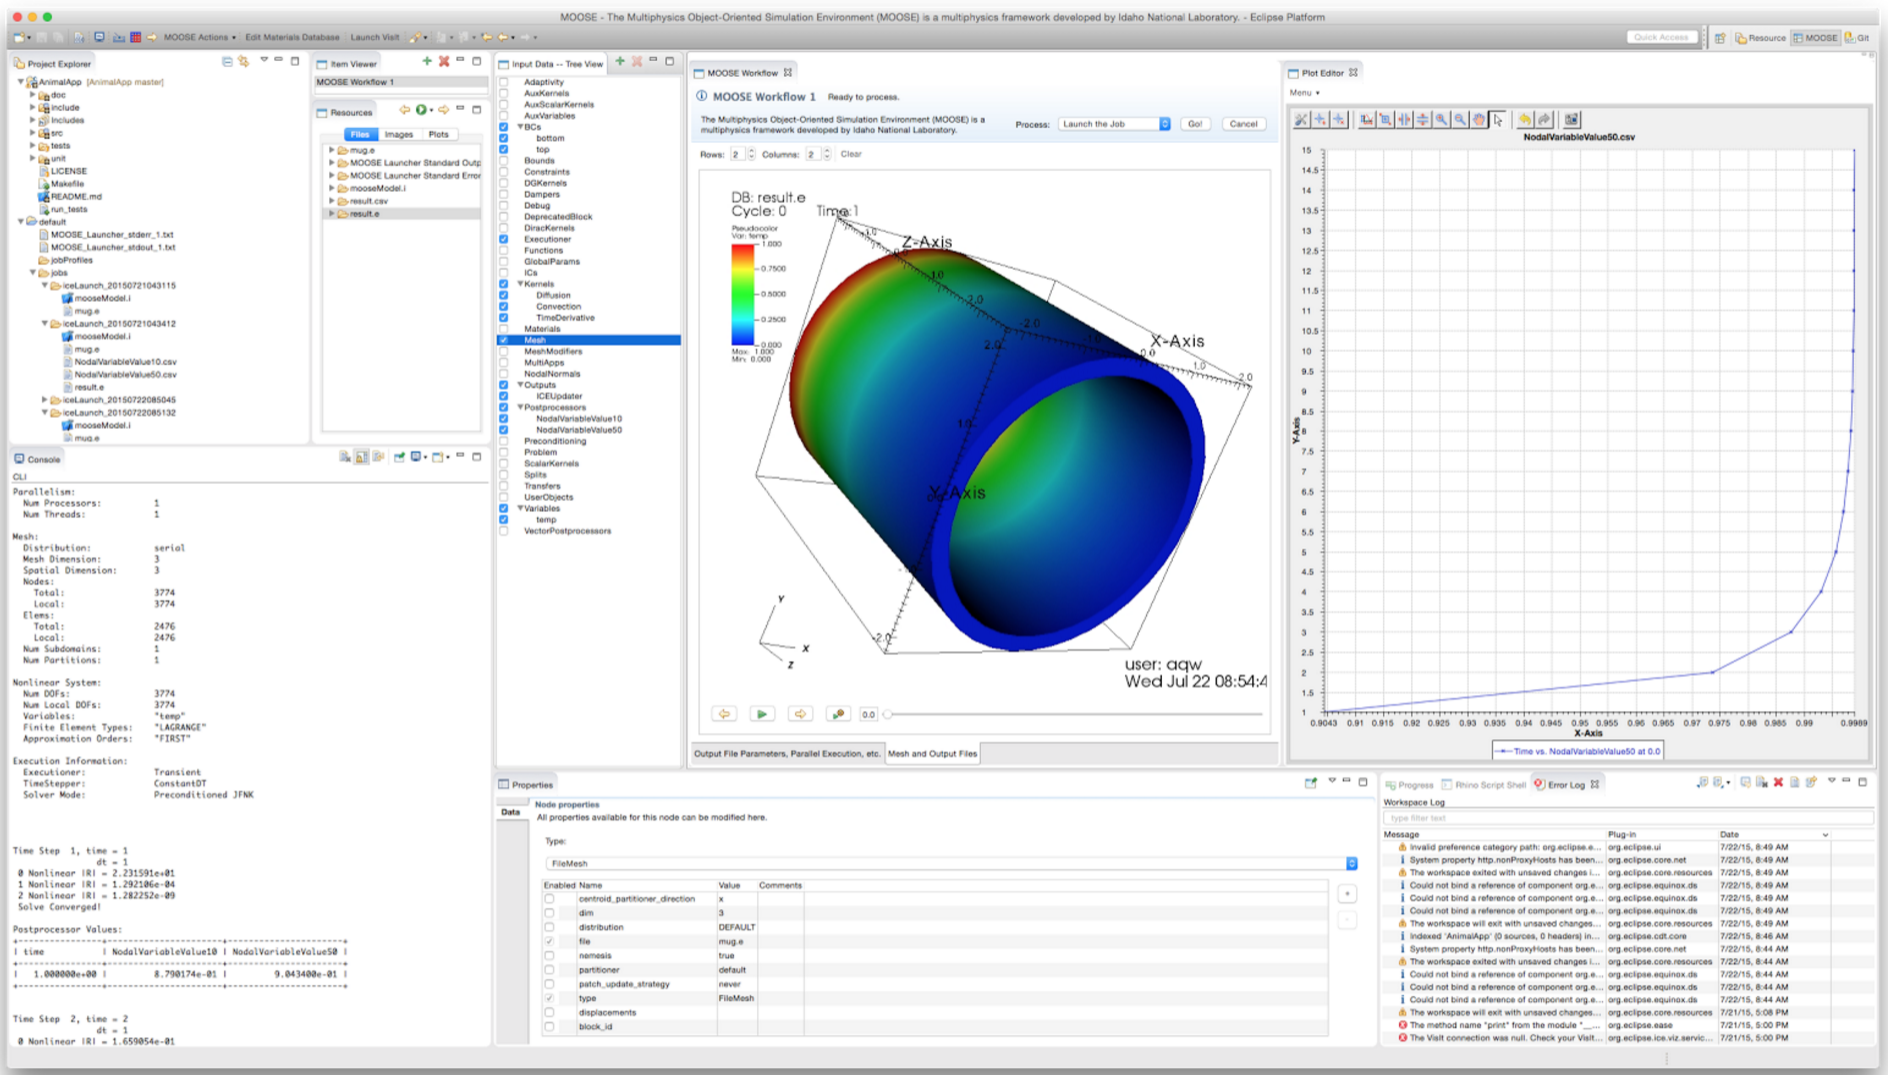
\includegraphics[width=\textwidth]{images/ice-moose.png}
\caption{ICE workbench for MOOSE workflows.}
\end{figure}

There are over three hundred MOOSE-based applications and it is very
easy to create new MOOSE applications. The ICE development team uses ICE
and MOOSE to quickly solve energy science problems with high-performance
computing resources and deploy domain specific workbenches. ICE includes
support for automatically downloading and building MOOSE from its GitHub
project, which then makes it possible to immediately begin developing
complex multiphysics applications using the Eclipse C Development Tools,
which are pre-installed in ICE to facilitate this interaction. Once the
new MOOSE-based application is built, it will automatically work with
the MOOSE workflow tools in ICE, although developers can also create
customized workflow tools as needed.

\subsection{Binder Jet Modeling}\label{binder-jet-modeling}

Solid-state sintering of parts printed using binder jetting
significantly increases part strength by decreasing the part porosity
and eliminating voids. The downside of this process is that it causes
the part to shrink and warp. An ideal near-net-shape process that
combined binder jetting with solid-state sintering would thus consider
warpage and deformation due to sintering in the design phase of the
part. Figure 3 shows an ICE-based workbench for performing simulations of
this process with visualizations of the pre- and post-simulation
properties of a central body with eight cantilevers. The primary
deformation in this type of geometry is bending or drooping of the
cantilevers, and ICE currently calls a custom MOOSE-based application
(which was written in ICE as described above) for simulating the
deformation of the cantilevers.

\begin{figure}[htbp]
\centering
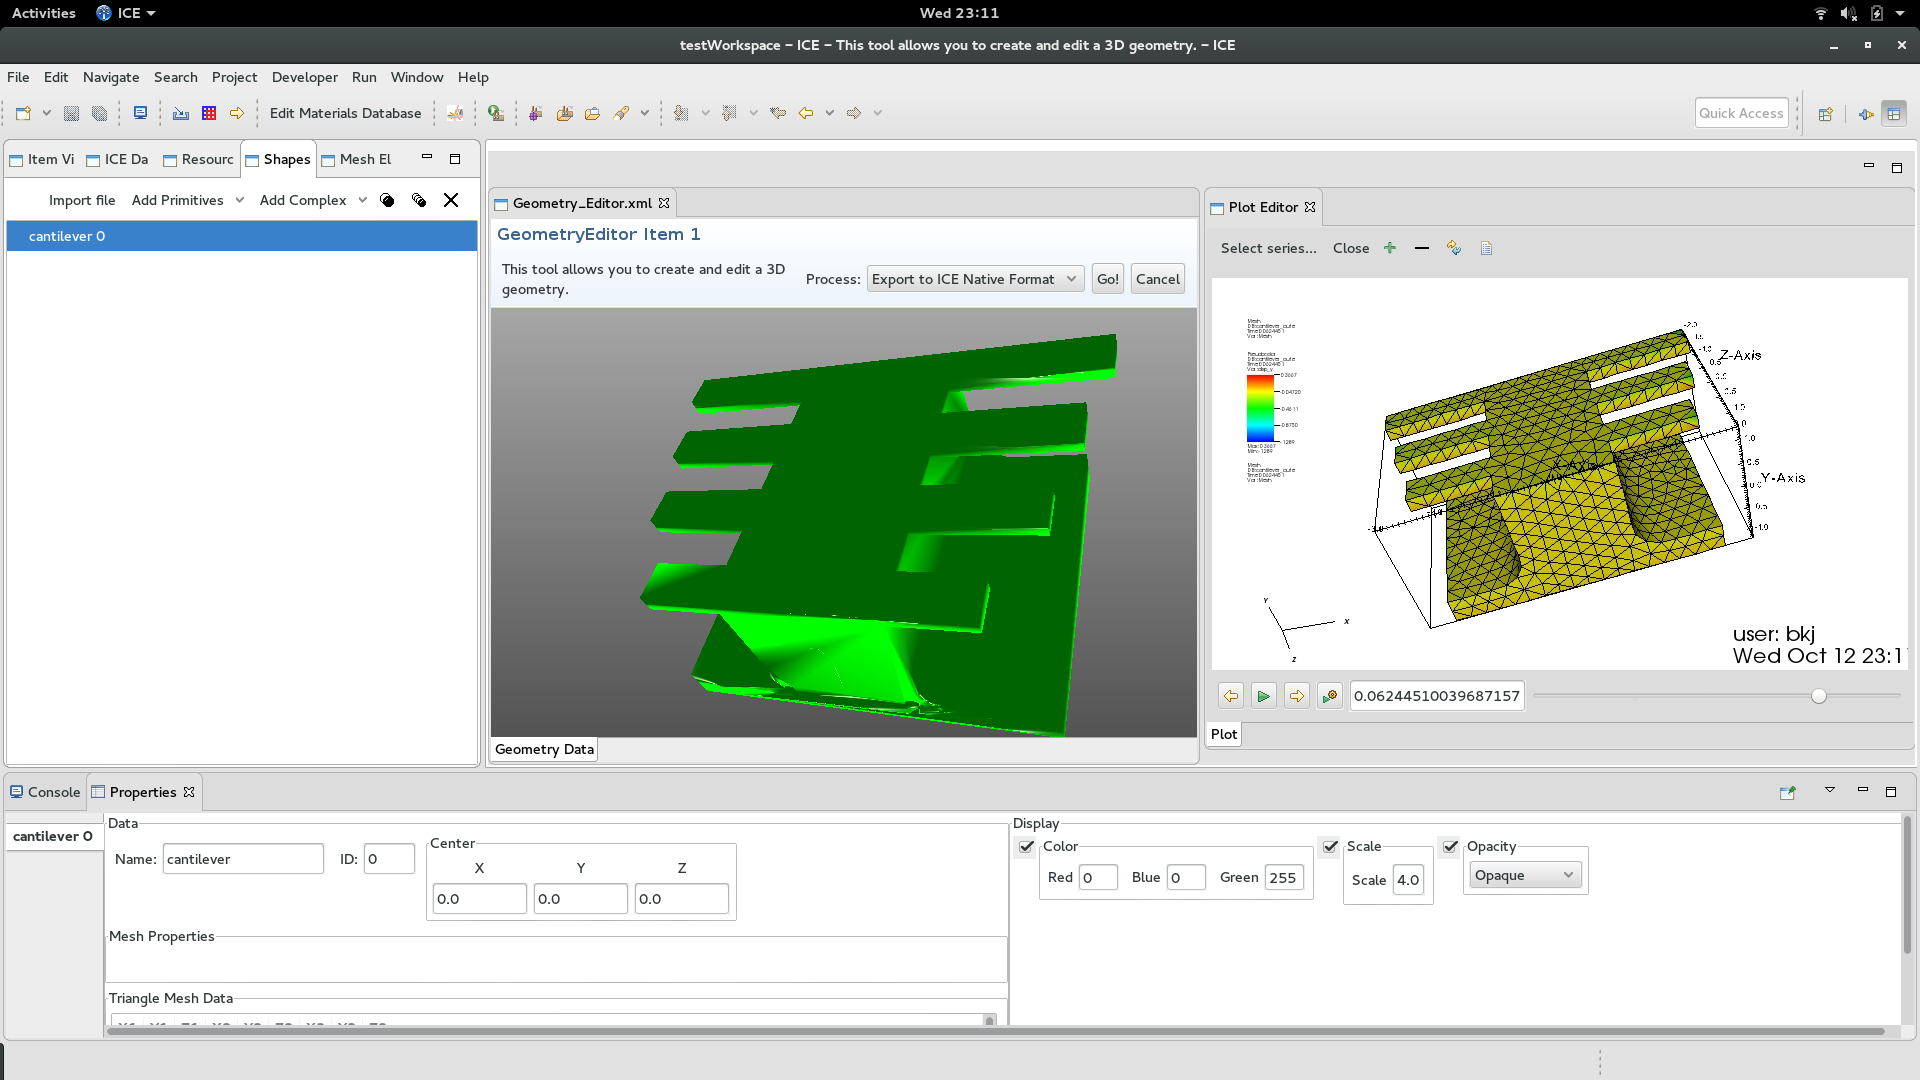
\includegraphics[width=\textwidth]{images/ice-bjm.png}
\caption{ICE workbench for binder jet modeling.}
\end{figure}

The full application for this work is expected to be released near the
end of 2017.

\subsection{Neutron Reflectivity}\label{neutron-reflectivity}

ICE includes a small utility for simulating neutron reflectivity and
comparing the results to data, \cite{billings_brand_2015}. This was developed
in collaboration with colleagues at the Spallation Neutron Source to
replace an older utility written in Visual Basic and distributed via
Excel macros. The newer utility in ICE is capable of processing a single
workflow and is shown in figure 4.

\begin{figure}[htbp]
\centering
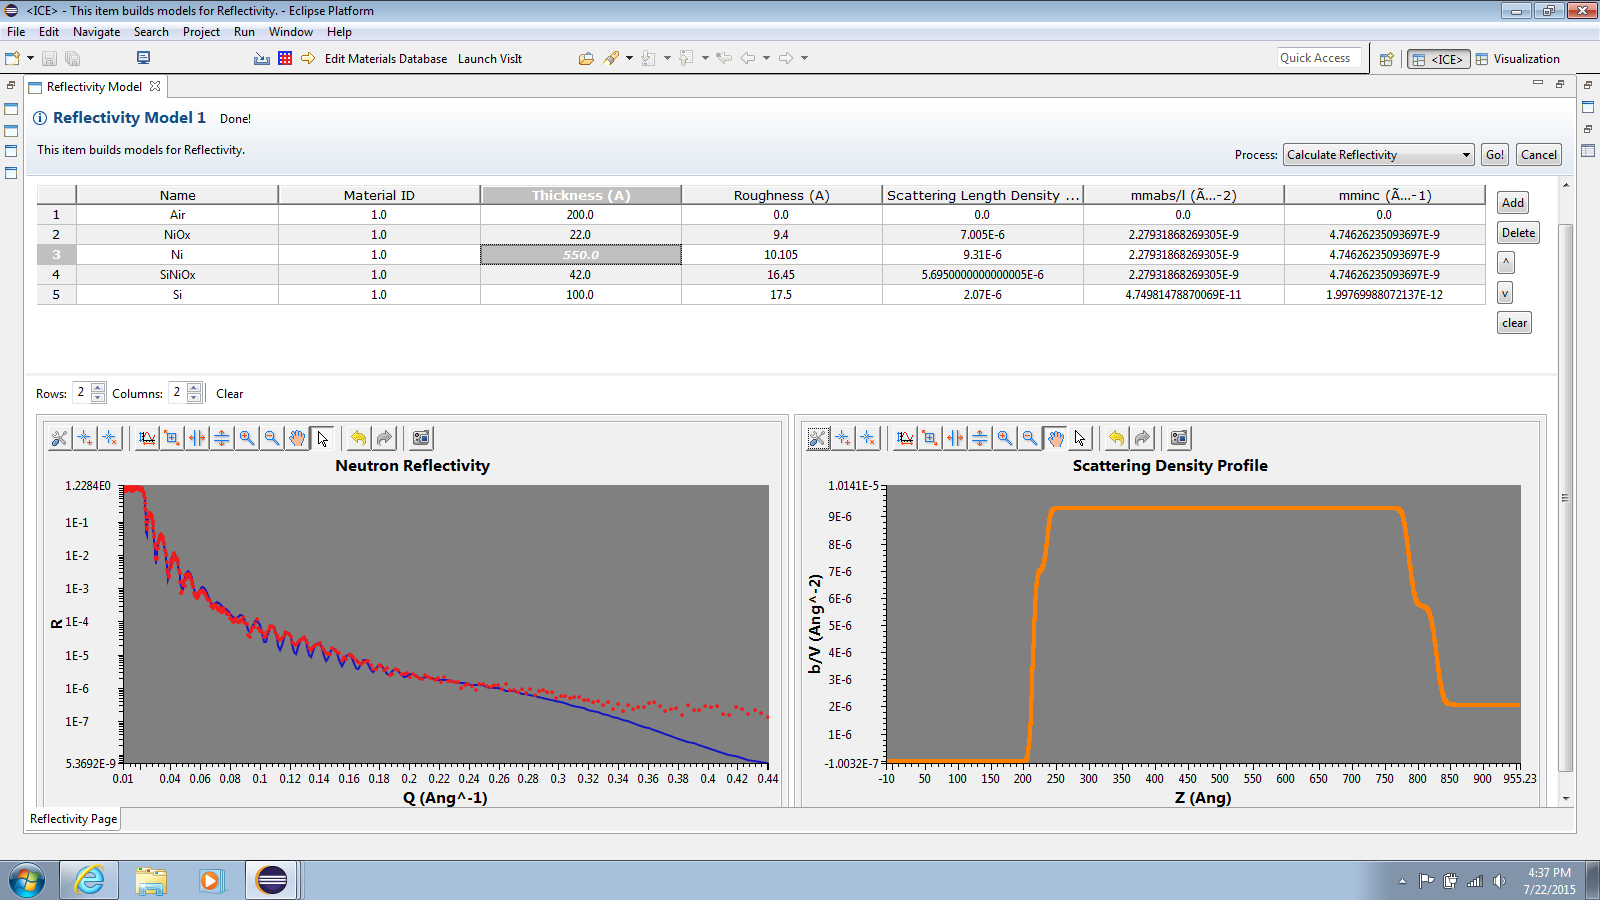
\includegraphics[width=\textwidth]{images/reflectivity-screenshot.png}
\caption{ICE workbench for neutron reflectivity.}
\end{figure}

\subsection{Quantum Computing}\label{quantum-computing}

As quantum computing grows, so too does the need for sophisticated
software that can utilize quantum hardware or perform calculations on
simulated quantum hardware. Humble et al. created a simulator for
adiabatic quantum computers where workflows were added to ICE to support
interaction with the simulator, but also to process large sets of
quadratic binary optimimzation problems, \cite{humble_integrated_2014}. Figure 5
shows the workbench for this project.

\begin{figure}[htbp]
\centering
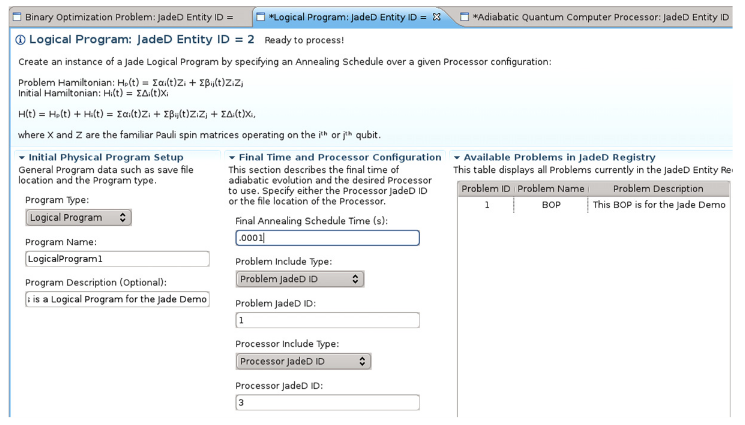
\includegraphics[width=\textwidth]{images/jaded.png}
\caption{ICE workbench in JADE for quantum computing simulations.}
\end{figure}

ICE also supports other quantum computing projects, including the
eXtreme-scale ACCelerator (XACC) programming framework,
\cite{mccaskey_ornl-qci/xacc_2016}. XACC is a programming framework for
extreme-scale, post-exascale accelerator architectures that integrates
alongside existing conventional applications.

\subsection{Nuclear Energy}\label{nuclear-energy}

There are many examples of ICE's role in modeling and simulation
projects for nuclear energy, but readers are referred to the work in
\cite{billings_domain-specific_2015} for an extreme example of the level of
customization that is possible in ICE. Support for the ``Reactor
Analyzer'' was dropped in ICE 2.1.8, but it demonstrated ICE's ability
to integrate many different nuclear energy tools for complex analysis.

\section{Impact}\label{impact}

The impact of software tools such as ICE are hard to quantify. However,
there are several places where ICE has significantly assisted its
development team and others.

One pressing area of interest and impact is that of interoperability
between workflow systems. There is significant prior art in combining
large workflow management systems, such as that Mandal et al.,
\cite{mandal_integrating_2007}, but the end goal of gaining the greatest
advantage by using the best capabilities from multiple systems remains elusive.
ICE's unique perspective on workflows and its well-defined API make it
possible to integrate multiple systems in a straightforward way. This
allows it to connect to other workflow environments, such as Triquetrum,
quite easily, \cite{brooks_introducing_2016}. Triquetrum, (like Kepler in
\cite{mandal_integrating_2007}), is a Ptolemy-based workflow engine,
\cite{brooks_triquetrum:_2015}. Several of the authors of this paper are using
it to investigate these issues.

It is widely known that tools that make researchers more productive tend
to improve the pursuit of existing research. The high extensibility of
ICE and the tools that it combines from the larger Eclipse ecosystem
have made it possible for researchers on the development team to quickly
deploy new simulation environments for problems, such as the binder jet
modeler and reflectivity tools mentioned earlier. Other tools created
with ICE may not radically invent something new, but they tend to
streamline interactions with those tools. Many ICE users (and certainly
the development team!) have experienced improvements in software
development activities because of the tools that ICE provides or learned
new technologies because access to new tooling was as simple as
installing more plugins through the Eclipse Marketplace.

The ICE development team does not track ICE's user base, as useful as
that would be, because of the extra work involved. However, various
sources such as the VIBE mailing list, ICE's own mailing lists, and
website download statistics suggest that ICE has been used by over 350
people at one time or another and currently has about twenty
``superusers,'' including the development team.

A new cloud based development tool based on ICE is under development by
RNET LLC out of Dayton, Ohio in response to an SBIR award from the U.S.
Department of Energy. This web based version of ICE will continue ICE's
support for nuclear energy and integrate with cloud services such as
Amazon Web Services and Oak Ridge National Laboratory's Compute and Data
Environment for Science (CADES). Additionally, while ICE has not led to
the development of ``spin-off'' companies, ICE source code has been used
in two spin-off projects: EAVP (mentioned earlier) for advanced
visualizations and the Eclipse January project for scientific data
structures, \cite{graham_eclipse_2016}. ICE was also one of the founding
projects of the Eclipse Science Working Group.

Eclipse ICE is an open source project and the authors welcome and encourage
engagement and contributions from readers. Interested parties may inquire by
contacting the corresponding author or visiting the website.

\section{Sample Code, Tutorials and Other
Resources}\label{sample-code-tutorials-and-other-resources}

The quintessential resource for information on ICE is the projects web
page, \cite{billings_eclipse_2016}. The ``Resources'' menu includes links to
detailed tutorials and documentation of multiple types. Examples of how to create
new workflow Items are available at
\url{https://github.com/eclipse/ice/tree/master/org.eclipse.ice.demo}.
Examples of how to use the scripting engine (in this case for neutron
reflectivity) are available at
\url{https://github.com/eclipse/ice/tree/master/examples}. ICE includes an
extensive test suite of unit, integration, and UI tests and these are
also excellent examples of how to work with the platform.

\section{Conclusions}\label{conclusions}

Workflows for computational scientists in modeling and simulation differ
greatly from experimentalists or those who primarily interact with
grid-based workflow management systems, which has driven the creation of
additional workflow management systems to meet those needs. This work 
presented the Eclipse Integrated Computational Environment (ICE) and 
described how it has been used to address interdisciplinary problems in 
modeling and simulation for energy science. Of particular note is the
difference in architecture between a workflow management system focused
on modeling and simulation compared to those focused on grids. ICE's broad
applicability across a number of topics in energy science suggests that
there are opportunities for these systems in general. Finally, one 
interesting avenue for future exploration is coupling or integrating ICE 
with other workflow tools such as Aiida, Triquetrum, Kepler and Pegasus,
which would make it possible to combine the best of grid and modeling and
simulation workflows to address greater challenges.

\section*{Acknowledgements}\label{acknowledgements}
\addcontentsline{toc}{section}{Acknowledgements}

The authors are grateful for the assistance and support of the following
people and institutions without which this work would not have been
possible. This includes many people who directly contributed to the
project, either in its early days as ``NiCE'' or once it moved to
Eclipse, including: Ronald Allen, Andrew Belt, Tim Bohn, David E.
Bernholdt, Erica Grant, Mike Guidry, Forest Hull, Eric J. Lingerfelt,
Sebastien Jourdain, JiSoo Kim, Allison Koenecke, Fangzhou Lin, Greg
Lyon, Tony McCrary, John M. Hetrick III, Elizabeth Piersall, Neeti
Pokhriyal, Adrian Sanchez, Claire Saunders, Nick Stanish, Matthew Wang,
Scott Wittenberg. The support of both the NEAMS and CASL programs is
greatly appreciated. The authors would like to acknowledge the special
contribution of the Eclipse Foundation, the Eclipse Community, the
Eclipse Science Working Group and our many colleagues who use and
contribute to open source projects in the Eclipse ecosystem.

Finally, the development team is especially grateful to Barney Maccabe,
David Pointer and John Turner of Oak Ridge National Laboratory for their
endless support and advocacy for this work.

This work has been supported by the US Department of Energy, Offices of
Nuclear Energy (DOE-NE) and Energy Efficiency and Renewable Energy
(DOE-EERE), and by the ORNL Undergraduate Research Participation
Program, which is sponsored by ORNL and administered jointly by ORNL and
the Oak Ridge Institute for Science and Education (ORISE). This work was
also supported in part by the Oak Ridge National Laboratory Director's
Research and Development Fund. ORNL is managed by UT-Battelle, LLC, for
the US Department of Energy under contract no. DE-AC05-00OR22725. ORISE
is managed by Oak Ridge Associated Universities for the US Department of
Energy under contract no. DE-AC05-00OR22750.

\section*{Required Metadata}\label{required-metadata}
\addcontentsline{toc}{section}{Required Metadata}

\section*{Current code version}\label{current-code-version}
\addcontentsline{toc}{section}{Current code version}

See Table \ref{codeTable}.

\begin{table*}[!htbp]
\begin{tabularx}{\textwidth}{|l|X|X|}
\hline
C1 & Current Code Version & `next'\tabularnewline\hline
C2 & Permanent link to code/repository used for this code version &
\url{https://github.com/eclipse/ice/tree/next}
\tabularnewline\hline
C3 & Legal Code License & Eclipse Public License 1.0 \tabularnewline\hline
C4 & Code versioning system use & Git \tabularnewline\hline
C5 & Software code languages, tools, and services used & Java, OSGi, Eclipse Rich Client Platform,
and Maven \tabularnewline\hline
C6 & Compilation requirements, operating environments \& dependencies & Java 1.8 or greater, Maven, and
an internet connection for dependencies \tabularnewline\hline 
C7 & If available Link to developer documentation/manual &
\url{https://wiki.eclipse.org/ICE} \tabularnewline\hline 
C8 & Support email for questions & ice-dev@eclipse.org \tabularnewline\hline
\end{tabularx}
\caption{Current Code Version}
\label{codeTable}
\end{table*}

\section*{Current executable software
version}\label{current-executable-software-version}
\addcontentsline{toc}{section}{Current executable software version}

See Table \ref{execTable}.

\begin{table*}[!htbp]
\begin{tabularx}{\textwidth}{|l|X|X|}
\hline
S1 & Current Code Version & 2.2.1 \tabularnewline\hline
S2 & ermanent link to executables of this version &
\url{https://www.eclipse.org/downloads/download.php?file=/ice/builds/2.2.1/}
 \tabularnewline\hline 
S3 & Legal Software License & Eclipse Public License 1.0 \tabularnewline\hline
S4 & Computing platforms/Operating Systems & Windows (32/64-bit), Mac OS/X,
Linux (32/64-bit) \tabularnewline\hline 
S5 & Installation requirements \& dependencies & Java 1.8 or
greater \tabularnewline\hline
S6 & If available, link to user manual - if formally published include a
reference to the publication in the reference list &
\url{https://wiki.eclipse.org/ICE} \tabularnewline\hline 
S7 & Support email for questions & ice-users@eclipse.org \tabularnewline\hline
\end{tabularx}
\caption{Current Executable Software}
\label{execTable}
\end{table*}